\documentclass{article}
\usepackage[hmargin=1in,vmargin=1in]{geometry}
\usepackage{listings}
\usepackage{color}
\usepackage{hyperref}
\usepackage{graphicx}
\usepackage{wrapfig}

% For better handling of unicode (Latin characters, anyway)
\IfFileExists{lmodern.sty}{\usepackage{lmodern}}{}
\usepackage[T1]{fontenc}
\usepackage[utf8]{inputenc}

\lstset{
    numbers=left,                   % where to put the line-numbers
    numberstyle=\small \ttfamily \color[rgb]{0.4,0.4,0.4},
                % style used for the linenumbers
    showspaces=false,               % show spaces adding special underscores
    showstringspaces=false,         % underline spaces within strings
    showtabs=false,                 % show tabs within strings adding particular underscores
    frame=lines,                    % add a frame around the code
    tabsize=4,                        % default tabsize: 4 spaces
    breaklines=true,                % automatic line breaking
    breakatwhitespace=false,        % automatic breaks should only happen at whitespace
    basicstyle=\ttfamily, %identifierstyle=\color[rgb]{0.3,0.133,0.133},   % colors in variables and function names, if desired.
    keywordstyle=\color[rgb]{0.133,0.133,0.6},
    commentstyle=\color[rgb]{0.133,0.545,0.133},
    stringstyle=\color[rgb]{0.627,0.126,0.941},
}

\hypersetup{
    colorlinks=true,
    linkcolor=blue,
    urlcolor=red,
    linktoc=all
}


\title{Rapport final de TIPE}
\author{PEREIRA Romain}
\date{4 Juin 2017}

\renewcommand*\contentsname{Sommaire}

\begin{document}

	\maketitle

	\tableofcontents

	\section*{Préambule}
		blblblblblblbl
	\newpage

	\section{Introduction}
		blblblblblblbl
	\newpage

	\section{Corps principal}
		\subsection{Modalités d'action}
			blblblblblblbl

		\subsection{Restitution des résultats}
			blblblblblblbl

			\begin{figure}
			\begin{center}
			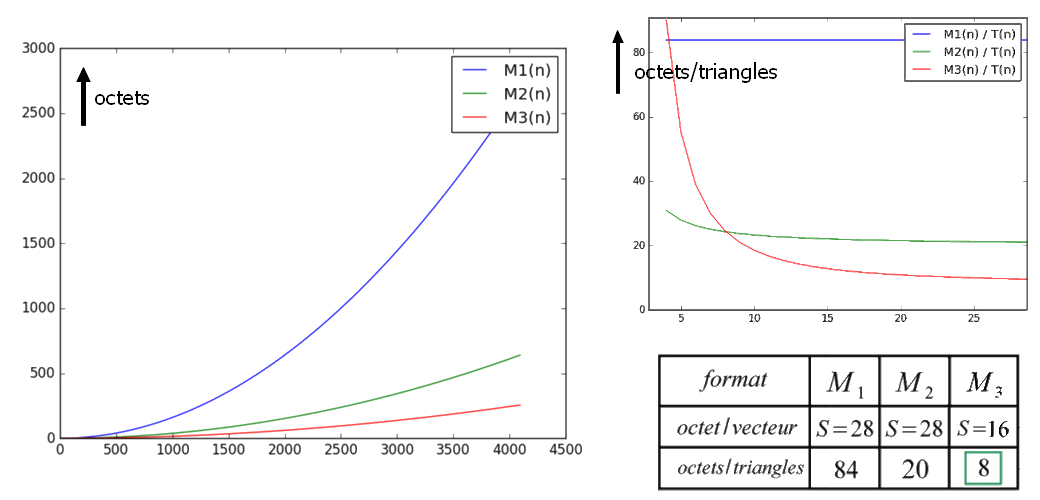
\includegraphics{../images/complexiteSpatial5.png} 
			\end{center}
			\caption{Utilisation mémoire du terrain \(n² est le nombre de point total)}
			\label{Utilisation mémoire du terrain}
			\end{figure}



		\subsection{Analyse - Exploitation - Discussion}
			blblblblblblbl
	\newpage

	\section{Conclusion générale}
		blblblblblblbl
	\newpage

	\section{Références}
		blblblblblblbl
	\newpage



\end{document}